\chapter{L'Architechture CORBA}

    \section{Qu'est ce que le cadre CORBA ?}

        \par CORBA est l’acronyme de \textit{\textbf{C}ommon \textbf{O}bject \textbf{R}equest \textbf{B}roker \textbf{A}rchitecture}. Il s’agit d’un standard développé en 1992 par Object Management Group (ou OMG) ; un consortium de plusieurs centaines d’entreprises dédiées à la construction de matériel informatique et l’édition de logiciels.\\
        L’objectif est de développer des applications distribuées indépendantes de la plate-forme et du langage à travers des principes de conception orientés objet.\\

        Corba repose sur la notion de bus logiciel (Object Request Broker).
        En Corba, tout est objet. On bénéficie donc des mécanismes d'héritage, polymorphisme et encapsulation.

    \section{Les avantages de Corba}

        \begin{itemize}[label= \ding{51}]
            \item \textbf{Interopérabilité: }Les objets Corba communiquent par l'intermédiaire du protocole IIOP (Internet Inter-ORB Protocol). Ce protocole permet la communication entre entités quelconques supportant le protocole TCP/IP.
            \item \textbf{Intégration aux systèmes existants: }Tout code existant peut être encapsulé dans un objet Corba (wrapping). Des passerelles existent pour des standards de distribution d'objets du marché (DCOM, DCE).
            \item \textbf{flexibilité du développement: }Les services rendus par les objets sont définis par leur interface qui tient lieu de contrat entre l'utilisateur et le fournisseur du service. Les parties définition et implantation d'un objet sont totalement dissociées.
        \end{itemize}

    \section{Objets distribués de CORBA}

        \begin{itemize}
            \item  Localisation indifférente dans le réseau;
            \item Sur des systèmes hétérogènes;
            \item Implantés dans des langages différents.
        \end{itemize}
\pagebreak
    
    \section{Composants logiciels}

        \begin{itemize}
            \item  Accédés par n'importe quel client;
            \item Via des invocations de méthodes;
            \item Le client ne connait que l'interface publiée par le serveur;
            \item L'interface est spécifiée dans un langage standard l'IDL.
        \end{itemize}

    \section{Le modèle objet client-serveur CORBA}

    Il est fondé sur une entité virtuelle, l'objet CORBA, gérée par le bus CORBA. Chaque application peut exporter ses services sous la forme d'objets CORBA.
    La coopération client-serveur se déroule de la manière suivante :
    \begin{enumerate}
        \item  Le client détient une référence sur un objet CORBA qui permet de le localiser sur le bus.
        \item Le client dispose de l'interface de l'objet CORBA (type abstrait de l'objet CORBA) qui définit ses opérations et ses attributs (exprimés dans le langage IDL).
        \item Le client réalise une requête (invoque) une opération sur l'objet CORBA.
        \item Le bus CORBA achemine cette requête vers l'objet CORBA tout en masquant les problèmes d'hétérogénéité liés aux langages, systèmes d'exploitation, machines, réseaux.
        \item L'objet CORBA est associé à un objet d'implantation
        \item Le serveur détient l'objet d'implantation qui code l'objet CORBA (cette implantation pouvant évoluer au cours du temps) et gère son état temporaire.
    \end{enumerate}
    \vfill

    \begin{figure}[h]
        \centering
        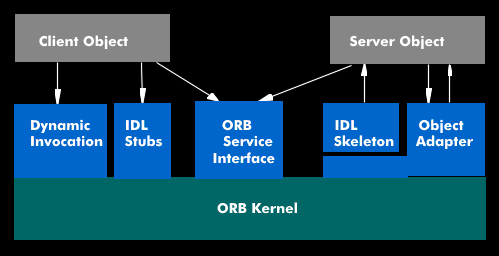
\includegraphics[scale= 0.77]{archiCorba/CORBA-Architektur.png}
        \caption{CORBA Architechtur}
    \end{figure}

    \section{Architecture CORBA}

        La relation entre objets distribués est une relation client-serveur. Le serveur fournit une interface distante. Le client invoque une interface distante. Le client peut lui-même jouer le rôle de serveur s'il implante une interface qui peut être invoquée à distance par d'autres objets. 
        \subsection*{Coté client}
        Le client connaît l'interface d'un objet spécifique (il dispose de l'IDL). Le client possède une représentation de l'objet distant appelée talon ("stub") générée par l'IDL. Le talon transmet la requête à l'objet distant via le bus logiciel (ORB). Il s'agit d'une représentation de l'objet distant responsable de la transmission d'une invocation de méthode du talon vers l'objet distant. Il ne s'agit pas d'une copie de l'objet distant.
            A travers le talon le client voit l'interface de l'objet sans savoir où est l'objet et sans connaître le langage de programmation utilisé pour son implantation.
            
            En pratique, le client :
            \begin{enumerate}
                \item créé une instance locale d'ORB
                \item récupère la référence du serveur de noms
                \item récupère la référence de l'objet
                \item invoque la méthode sur l'objet distant
            \end{enumerate}
        \subsection*{Coté serveur}
            L'ORB utilise un squelette de code pour traduire l'invocation distante en un appel de méthode sur l'objet local. Le squelette traduit l'appel et les paramètres dans le format de l'implantation spécifique et appelle la méthode invoquée.
            Au retour de la méthode, les résultats ( ou erreurs ) sont traduits par le squelette et renvoyés au client via l'ORB.
            Communication entre ORB, protocoles réseaux
            Tout bus à la norme CORBA 2.0 doit fournir les protocoles GIOP et IIOP.
            
            GIOP est un protocole générique. Il fournit :
            \begin{itemize}[label= $\bullet$]
                \item une représentation commune des données : CDR (Common Data Representation)
                \item un format de référence d'objet interopérable : IOR (Interoperable Object Reference)
                \item un ensemble de messages de transport de requêtes aux objets (request, reply, ...)
            \end{itemize}

            \par Les ORBs partagent un protocole commun IIOP ((Internet Inter ORB Protocol), implantation de GIOP sur TCP/IP et donc de l'internet. Ce protocole définit comment les ORBs (répondant à la spécification CORBA) se transmettent de l'information.\\
            
            Autres services fournis par les ORBs :
            \begin{itemize}[label= $\bullet$]
                \item Recherche d'objets par leur nom
                \item Maintenance d'objets persistants
                \item Support pour le traitement transactionnel ...
            \end{itemize}

            

    
    